\documentclass[11pt,a4paper]{article}
%\usepackage[pdftex]{graphicx,color}
\usepackage{graphicx,color}
\usepackage{amsmath,amssymb,dsfont,fullpage,epsfig,multirow,longtable,bm}
\usepackage{epsfig,epstopdf,hhline}
\usepackage{cases}
\usepackage{wrapfig}
\usepackage{algorithm}
%\usepackage[noend]{algorithmic}
\usepackage{algorithmic}
\renewcommand{\algorithmicrequire}{\textbf{Input:}}
\renewcommand{\algorithmicensure}{\textbf{Output:}}
%\usepackage[numbers]{natbib}
\usepackage[top=1 in, bottom=1 in, left=1 in, right=1 in, letterpaper]{geometry}
\usepackage{tikz}
\usetikzlibrary{arrows,positioning,decorations.pathreplacing,shapes}

\usepackage{thmtools}
\usepackage{thm-restate}
\usepackage{enumerate}

% Ours
\usepackage{mdframed}
\usepackage{setspace}
\usepackage{caption}
\usepackage{xfrac}

%\declaretheorem[name=Theorem]{thm}

% for affiliation
\usepackage{authblk}

%%%%%%%%%% Start TeXmacs macrosƒ
\newenvironment{proof}{\noindent\emph{Proof\ }}{\hspace*{\fill}$\Box$\medskip}
\newenvironment{claimproof}{\noindent\emph{Proof of claim\ }}{\hspace*{\fill}$\Box$\medskip}
\newenvironment{plainproof}{\noindent\emph{Proof\ }}{}
\newtheorem{theorem}{Theorem}
\newtheorem{definition}{Definition}
\newtheorem{lemma}{Lemma}
\newtheorem{claim}{Claim}
\newtheorem{proposition}{Proposition}
\newtheorem{corollary}{Corollary}
\usepackage{amsmath}
\usepackage{paralist}
\usepackage{framed}

%%comment in algorithms
\renewcommand{\algorithmiccomment}[1]{\hfill  {\small  \tt \# #1}}

\newcommand\restr[2]{{% we make the whole thing an ordinary symbol
  \left.\kern-\nulldelimiterspace % automatically resize the bar with \right
  #1 % the function
  \vphantom{\big|} % pretend it's a little taller at normal size
  \right|_{#2} % this is the delimiter
  }}

\newcommand{\vect}[1]{\ensuremath{\bm{#1}}}
\newcommand{\one}{\ensuremath{\mathds{1}}}
\newcommand{\SW}{\textnormal{SW}}

\newcommand{\pred}{\texttt{pred}}
\newcommand{\PoA}{\text{PoA}}
\newcommand{\E}{\ensuremath{\mathbb{E}}}
% bullet dot
\newcommand\sbullet[1][.75]{\mathbin{\vcenter{\hbox{\scalebox{#1}{$\bullet$}}}}}

\usepackage[utf8]{inputenc} % Required for inputting international characters
\usepackage[T5]{fontenc} % Output font encoding for international characters

\usepackage{color, colortbl}
\usepackage{hyperref}
\hypersetup{colorlinks,
            linkcolor=blue,
            citecolor=blue,
            urlcolor=magenta,
            linktocpage,
            plainpages=false}
\usepackage[capitalise,noabbrev]{cleveref}

\usepackage[numbers]{natbib}

\newcommand{\comment}[1]{\textcolor{blue}{{\footnotesize
#1}}\marginpar{\raggedright\tiny \textcolor{blue}{Comment}}}


\begin{document}

\title{The Price of Anarchy bound of 2 is tight for efficient welfare for proportional allocation}

\author{Kevi Enik\H{o}}
\author{Nguyễn Kim Thắng}
\affil{LIG, University Grenoble-Alpes, France }

\maketitle

\begin{abstract}
    Auctions with divisible resources represent various practically relevant problems, such as network bandwidth allocation and food aid distribution. In each of these settings, the desire to receive (or the need of) a resource is represented by bids. The proportional allocation mechanism assigns a fraction of the resource to each bidder in proportion to the bid across all the bids. Despite the importance of these type of auctions, the efficiency of proportional allocations is still not completely understood. In recent years, \cite{Tardos2013} proved a lower bound of $26.8\%$ for the Price of Anarchy (PoA) considering social welfare, and \cite{Caragiannis2014} improved their analysis to $50\%$ both for social and effective welfares. This paper follows a different perspective on the analysis of this problem, which relies on the primal-dual method (first introduced in this setting by \cite{Thang2017}). We prove that the Price of Anarchy (PoA) bound considering the effective welfare of proportional allocation over coarse-correlated and Bayes-Nash equilibria in the complete information setting for a single item is $50\%$, and this result is \emph{tight}.
\end{abstract}
%!TEX root = ./main.tex

\section{Introduction}

% Introduction and motivation for our problem
% main objective: compare the best combination of experts.
% So for in the literature, always compare to the best expert (ex., regret)

The domain of algorithms with predictions \cite{MitzenmacherVassilvitskii20:Beyond-the-Worst-Case}  (or learning-augmented algorithms) emerged recently and grew immensely at the intersection of (discrete) algorithm design and machine learning (ML).
Combining ML techniques with traditional algorithm design methods enables online algorithms to benefit from predictions that can infer future information from patterns in past data. Online algorithms with predictions can obtain performance guarantees beyond the worst-case analysis and provide fine-tuned solutions to various problems. In the literature, many significant problems have new learning-augmented results, for example, scheduling \cite{LattanziLavastida20:Online-scheduling,Mitzenmacher20:Scheduling-with}, caching (paging) \cite{LykourisVassilvtiskii18:Competitive-caching,Rohatgi20:Near-optimal-bounds,AntoniadisCoester20:Online-metric}, ski rental \cite{GollapudiPanigrahi19:Online-algorithms,KumarPurohit18:Improving-online,AngelopoulosDurr20:Online-Computation}, counting sketches \cite{HsuIndyk19:Learning-Based-Frequency}, bloom filters \cite{KraskaBeutel18:The-case-for-learned,Mitzenmacher18:A-model-for-learned}, and metrical task systems \cite{AntoniosEtAll23:mixing-predictions-metric-algorithms}.

Even though predictions provide a glimpse of the future, there is no mathematical guarantee for their accuracy. Adjusting the algorithm's trust in the predictions is a significant challenge since online algorithms must make irrevocable decisions at each time step. Ideally, if the predictions are accurate, the algorithm should perform well compared to the offline setting. In contrast, if the predictions are misleading, the algorithm should maintain a competitive solution, similar to the online setting where no predictive information is available. In other words, online algorithms with predictions are expected to bring the best of both worlds: mathematical performance guarantees of classical algorithms and good future prediction capabilities of machine learning methods.

Predictions can come from multiple sources (for example: heuristics, oracles, and randomized methods), but we ignore their nature and call all of them \emph{experts}.  An algorithm's consistency with the experts' suggestions is typically measured by comparing the algorithm's result with the solution of the \emph{best} expert. A representative example is the popular notion of regret in online learning, which fueled the development of many powerful algorithms and techniques.

A natural research question is whether it is possible to design competitive algorithms with mathematical performance guarantees with a stronger benchmark than the best expert. Comparing an algorithm with a stronger benchmark could provide deeper insights into the learning process and give better ways of exploiting the experts' predictions.

Taking a broader view, we can study whether combining predictions of several experts is similar to combining multiple online algorithms and whether we can expect to achieve better solutions with the combination. Assuming that we do not know in advance which of the given algorithms would perform best on the upcoming requests, can we combine the algorithms in some generic way to obtain a competitive online strategy? This has been a long-standing question in the community of online algorithms \cite{AzarBroder93:On-line-Choice,BlumBurch00:On-line-Learning}. To find an answer, it is a crucial to understand to what extent such an online strategy can benefit from the input of multiple algorithms and what is a suitable benchmark to evaluate its performance.

While in a completely general setting such an online strategy and a corresponding benchmark may not exist, in this paper we propose
two algorithms for online linear and convex problems with covering constraints that are competitive with the new benchmark (informally the \emph{best linear combination} of the experts). Therefore, our paper partially addresses the question we raised in the previous paragraph.

\subsection{Model and Problem}

\paragraph{Covering problem with experts.}
In the linear problem setting, we have $n$ resources and each resource $i$ has a cost per unit $c_{i}$ that we know in advance ($1 \leq i \leq n$).
Let $x_{i}$ be a non-negative variable representing the amount chosen from resource $i$.
The total cost of a solution $(x_{i})_{i=1}^{n}$ is $\sum_{i=1}^{n} c_{i} x_{i}$.
The problem includes $K$ experts and the problem's covering-type constraints are revealed online one-by-one.
At each time $t \geq 1$, we receive a covering constraint $\sum_{i=1}^{n} a_{i}^{t} x_{i} \geq 1$ (where $a_{i}^{t} \geq 0$) and each expert $k$ (where $1 \leq k \leq K$) provides
a solution $(s_{i,k}^{t})_{i=1}^{n}$. Our algorithm can observe the experts' solutions and afterwards it must update its own solution (denoted as $(x_{i}^{t})_{i=1}^{n}$)
to satisfy the new constraint, while maintaining the satisfaction of the previous ones. This algorithm must update its solution in the sense of online algorithms, so it cannot modify the previously made decisions. Formally, $x_{i}^{t} \geq x_{i}^{t-1} ~\forall\ i, t$.
Our goal is to design an algorithm that minimizes $\sum_{i=1}^{n} c_{i} x_{i}^{T}$ subject to
all online covering constraints $t$, where $1 \leq t \leq T$. The value $T$ is the last time a constraint is released, and it is not known by the algorithm.

The convex problem setting is analogous to the linear one, since we consider convex problems with linear constraints. The only difference compared to the previous paragraph is the total cost of the solution $(x_{i})_{i=1}^{n}$, which becomes $f(x)$, where $f$ is a convex function.

\paragraph{Experts.} \label{subsec:experts} In our model, the experts' predictions are also online solutions. In other words, the experts' solutions
fulfill the following properties:
\begin{enumerate}
	\item for every expert $k$ and for every time $t$ the solution $(s_{i,k}^{t})_{i=1}^{n}$ is feasible, therefore, every constraint $t'$ where $1 \leq t' \leq t$ is satisfied;
	\item for every expert $k$ and for every time $t$ and for every resource $i$, the previous expert solutions are irrevocable, therefore $s_{i,k}^{t} \geq s_{i,k}^{t'}$ for all $t' \leq t$.
\end{enumerate}
These properties can be verified online. If some experts do not satisfy them, we simply ignore those experts both in the decision-making and in the benchmark.
A crucial remark: we do \emph{not} assume that the experts' solutions are tight at each constraint $t$, requiring $\sum_{i=1}^{n} a_{i}^{t} s_{i,k}^{t} = 1 ~ \forall t, k$ to hold.
This assumption is unrealistic and cannot be maintained in an online manner (see the discussion in Appendix~\ref{appix-tight-solutions}).
Besides, assuming tight constraint satisfaction would simplify the problem, while intuitively,
the difficulty of designing competitive algorithms comes from the lack of obvious ways to distinguish
good expert solutions from (probably many) non-efficient/misleading ones.

\paragraph{Benchmark.}
We consider a dynamic benchmark that captures the \emph{best linear combination} of all experts' solutions \emph{over time}.
Informally, at any online time step, the benchmark can take a linear combination of the experts' solutions.
The linear combination can be changed over time, and it can be different from previous combinations.
However, the benchmark's decisions are also online, so it cannot decrease the value of the decision variables ($x_{i}$).
We refer to our benchmark with the name \texttt{LIN-COMB} from now on.

The \texttt{LIN-COMB} benchmark's formal description is visible on \cref{fig:benchmark}.
Let $w_{k}^{t} \geq 0$ be the weight assigned by the \texttt{LIN-COMB} benchmark to expert $k$ (where $1 \leq k \leq K$) at time~$t$.
Since we consider a linear combination, the constraint $ \sum_{k=1}^{K} w_{k}^{t} = 1$ must hold.
%In the linear program, we consider the relaxed version of this constraint, where $\sum_{k=1}^{K} w_{k}^{t} \geq 1$.
The solution of \texttt{LIN-COMB} at time $t$ is ideally $x_{i}^{t} = \sum_{k=1}^{K} w_{k}^{t} s_{i,k}^{t}$,
however, $x_{i}^{t}$ must be larger than $x_{i}^{t-1}$.
Therefore, we set $x_{i}^{t} = \max\bigl\{\sum_{k=1}^{K} w_{k}^{t} s_{i,k}^{t},\ x_{i}^{t-1}\bigr\}$.
In other words, given the chosen weights, if  $\sum_{k=1}^{K} w_{k}^{t} s_{i,k}^{t} < x_{i}^{t-1}$ then $x_{i}^{t} \gets x_{i}^{t-1}$,
otherwise $x_{i}^{t} \gets \sum_{k=1}^{K} w_{k}^{t} s_{i,k}^{t}$.

\begin{figure}[ht]
	\begin{mdframed}
	%	\begin{spacing}{0.1}
		\begin{align*}
			\text{Linear objective:} && \min \sum_{i=1}^{n} c_{i} x_{i}^{T} &= \min \sum_{i=1}^{n} c_{i} \sum_{t=1}^{T}\bigl( x_{i}^{t} - x_{i}^{t-1}\bigr)\\
			\text{Convex objective:} && \min f(x^{T}) &\\
	%	\end{align*}
	%	subject to
	%	\end{spacing}
	%	\begin{align*}
		&& & \\
		\text{Subject to (in both cases):} &&
			\sum_{k=1}^{K} w_{k}^{t} &= 1  && \forall\ t \\
			%
			&& x_{i}^{t} &\geq \sum_{k=1}^{K} w_{k}^{t} s_{i,k}^{t} && \forall\ i, t\\
			%
			&& x_{i}^{t} &\geq x_{i}^{t-1} && \forall\ i, t\\
			%
			&& w_{k}^{t} &\geq 0  && \forall\ t, k
		\end{align*}
		where $1 \leq t \leq T$, $1 \leq i \leq n$, and $f$ is convex.
		\vspace{5pt}
	\end{mdframed}
	\caption{Formulation of the \texttt{LIN-COMB} benchmark for both the linear and convex problems}
	\label{fig:benchmark}
	\end{figure}

Since every expert's solution is feasible by our assumptions, at each time $t$ and for all resource $i$ (where $1 \leq i \leq n$),
the constructed solution $x_{i}^{t} \geq \sum_{k=1}^{K} w_{k}^{t} s_{i,k}^{t}$ constitutes a feasible solution to the covering constraints of the original covering problem.
Formally, for every constraint $t'$ with $t' \leq t$,
%
\begin{align*}
\sum_{i=1}^{n} a_{i}^{t'} x_{i}^{t} \geq
%
\sum_{i=1}^{n} a_{i}^{t'} \biggl( \sum_{k=1}^{K} w_{k}^{t} s_{i,k}^{t} \biggr)
%
	= \sum_{k=1}^{K} w_{k}^{t}  \biggl( \sum_{i=1}^{n} a_{i}^{t'} s_{i,k}^{t} \biggr)
%
	\geq \sum_{k=1}^{K} w_{k}^{t} \geq 1
\end{align*}
%
where the second inequality holds due to the feasibility of the experts' solutions.
%
%Let $y_{i}^{t}$ be a variable representing the increase of $x_{i}^{t}$ compared to $x_{i}^{t-1}$. The benchmark is as follows.
%%
%\begin{align*}
%    && \min \sum_{t = 1}^{T} \sum_{i=1}^{n} & c_i y_i^t \\
%%
%    (\alpha^{t}) \qquad && \sum_{k=1}^{K} w_{k}^{t} & \geq 1  & \forall\ 1 \leq t \leq T,\ 1 \leq i \leq n \\
%%
%    (\beta_{i}^{t}) \qquad && \sum_{k=1}^{K} \left(w_{k}^{t} s_{i,k}^{t} - w_{k}^{t-1} s_{i,k}^{t-1} \right) &\leq y_i^t  &\forall\ 1 \leq t \leq T,\ 1 \leq i \leq n\\
%%
%    && w_{k}^{t},\ y_{i}^{t} & \ge 0 & \forall\ 1 \leq t \leq T,\ 1 \leq i \leq n,\ 1 \leq k \leq K
%\end{align*}
%
We highlight that the best-expert benchmark is included in \texttt{LIN-COMB}. We get the solution of this benchmark by setting $w^{t}_{k^{*}} = 1$ for all $t$, where $1 \leq t \leq T$, and $w^{t}_{k} = 0$ for all $k \neq k^{*}$,
where $k^{*}$ is the best expert (so $x_{i}^{t} = s_{i,k^{*}}^{t}$ for all $i$ and $t$).

\subsection{Our approach and contribution}

\paragraph{Approach.} We use the primal-dual approach to design competitive algorithms with the new \texttt{LIN-COMB} benchmark. First, we relax the linear program formulation of \texttt{LIN-COMB}, which serves as a lower bound. Then, we take the dual of the relaxation, which is a lower bound on the relaxation. Therefore, following the chain of lower bounds, the dual problem is a lower bound on the \texttt{LIN-COMB} benchmark. The formulations of the relaxation and its dual is detailed in \cref{sec:covering} for linear problems and in \cref{sec:convex} for convex problems.

Both of our proposed algorithms set the decision variables at every time step based on the solution of an internal convex program. Our approach is inspired by the
convex regularization method of \cite{BuchbinderChen14:Competitive-Analysis}, where the objective of the convex program is a shifted entropy function.
These functions have been widely used, in particular in the recent breakthrough related to $k$-server \cite{BubeckCohen18:K-server-via-multiscale,BuchbinderGupta19:k-servers-with}
and metrical task system problems \cite{BubeckCohen21:Metrical-task},
in which the entropy functions are shifted by constant parameters.

\paragraph{Novelty.} A novel point in our approach is that the entropy function is shifted by the average of the experts' solutions.
Moreover, regarding the constraints of the convex program, instead of using the experts' solutions directly,
we define auxiliary solutions that guarantee tight constraint satisfaction. We only use these tight solutions in the constraints and they play a crucial role in the proofs.

\paragraph{Results.} Let $\rho$ be the maximum ratio between the experts' solutions on the resources. Formally,
%We define the following parameter to establish the competitive ratio of our algorithm.
\[
	\rho := \max_{i} \max_{t',t''} \biggl\{\frac{\sum_{k=1}^{K} s_{i,k}^{t'}}{\sum_{k=1}^{K} s_{i,k}^{t''}} \biggr\}  \textnormal{ s.t. } \sum_{k=1}^{K} s_{i,k}^{t''} > 0.
\]
Informally, $\rho$ represents the discrepancy across the experts' predictions.
Our main result consists of two algorithms. The first one (which provides solutions for online linear covering) has an objective cost at most $O(\ln(K\rho))$ times the cost of the \texttt{LIN-COMB} benchmark. The second one (for online convex covering) achieves an objective cost at most $O(\ln(K\rho)) \cdot \frac{\lambda}{(1-\mu\ln(K\rho))}$ times the cost of \texttt{LIN-COMB}, where $\lambda$ and $\mu$ are the ($\lambda$,$\mu$)-smoothness parameters of the objective function.
In particular, for $0$-$1$ optimization problems, where the experts provide integer (deterministic or randomized) solutions, our first algorithm is $O(\ln(K))$-competitive with \texttt{LIN-COMB}, and the second one is $O(\ln(K)) \cdot \frac{\lambda}{(1-\mu\ln(K))}$-competitive.
An interesting feature of our algorithms is their resilience to the fluctuation of the quality of predictions (discussed in \cref{subsec:related-works} and illustrated with experiments in \cref{sec:exp}).

\subsection{Related work and discussions} \label{subsec:related-works}

Much of the research focusing on surpassing worst-case performance guarantees is motivated by the spectacular advances of machine learning (ML). Specifically, ML methods can detect patterns among the arriving input requests and provide valuable insights for the online algorithms regarding future requests. \cite{LykourisVassilvtiskii18:Competitive-caching} introduced a general framework to integrate ML predictions into classical algorithm designs to surpass the worst-case performance limit.
As a result, many practically relevant online problems were revisited to enhance existing classical algorithms with ML predictions (see the aforementioned \cite{LattanziLavastida20:Online-scheduling,Mitzenmacher20:Scheduling-with,LykourisVassilvtiskii18:Competitive-caching,Rohatgi20:Near-optimal-bounds,AntoniadisCoester20:Online-metric,GollapudiPanigrahi19:Online-algorithms,KumarPurohit18:Improving-online,AngelopoulosDurr20:Online-Computation,HsuIndyk19:Learning-Based-Frequency,KraskaBeutel18:The-case-for-learned,Mitzenmacher18:A-model-for-learned,AntoniosEtAll23:mixing-predictions-metric-algorithms}).

On a high-level view, we aim to design algorithms that are robust (competitive) to the offline optimal solution and also consistent with the expert's predictions. Ideally, the performance of the designed algorithm should surpass previous bounds whenever the predictions are reliable (low errors).
However, most learning-augmented algorithms suffer when the error rates are neither very low nor very high, resulting in prediction confidence that is neither very low nor very high.
Figure~\ref{fig:robustness-consistency} provides a general picture of the performance of an algorithm with predictions, which is representative for many problems (for example, \cite{BamasMaggoriSvensson20:primal-dual-method,KeviNguyen23:Primal-Dual-Algorithms}).

\begin{wrapfigure}{r}{0.4\textwidth}
	\vspace{-1.2cm}
	\begin{center}
		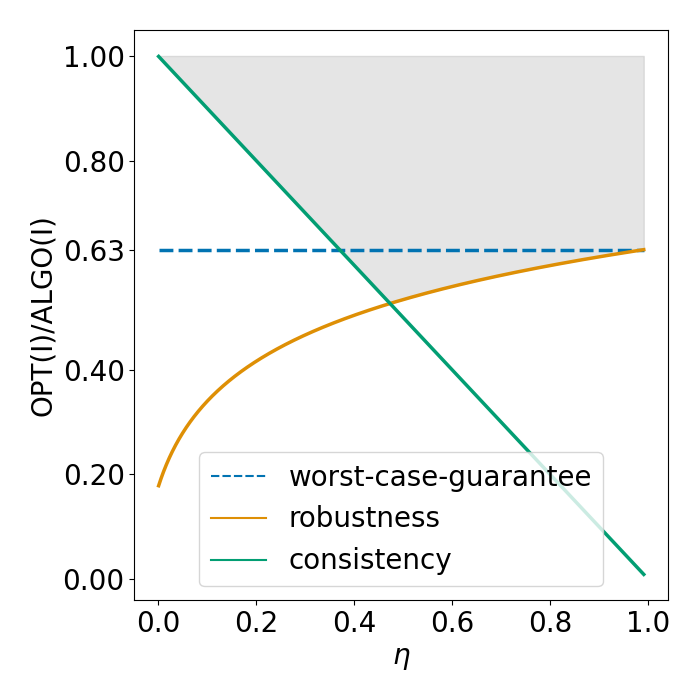
\includegraphics[width=0.4\textwidth]{../paper/Img/consistency_robustness.png}
	\end{center}
	\vspace{-1cm}
	\caption{Robustness-Consistency}
	\label{fig:robustness-consistency}
	\vspace{-0.2cm}
\end{wrapfigure}

\noindent In the figure, $\eta$ indicates the confidence in the predictions (or equivalently the error rate of predictions). The learning-augmented algorithm's performance bound is the maximum value of the green and orange curves (gray shaded area on the figure). We can observe that when $0.4 \leq \eta \leq 0.9$,
the algorithm's performance guarantee is worse than the classical worst-case guarantee (that can be achieved by simply ignoring all predictions).
Intuitively, in the case of neither very low nor very high confidence in the predictions, the algorithm has a hard time deciding if it should follow the predictions or the best-known standard algorithm in the worst-case paradigm.
It naturally raises the question whether we can achieve at least a constant factor of the worst-case guarantee (where the constant is as close to 1 as possible), while assuring a resilient output solution regardless of the predictions' quality.
Our algorithms with the new benchmark provides an answer to this question.


The paper of \cite{AnandGe22:Online-Algorithms} is the closest to ours, which also studies the design of algorithms with multiple experts.
They consider a \texttt{DYNAMIC} benchmark that is intuitively
the minimum cost solution that is supported by at least one expert solution at each time step. Formally:
\[\texttt{DYNAMIC} = \min_{\hat{\textbf{x}} \in \hat{X}} \sum_{i=1}^{n} c_i \hat{x}_i \textnormal{, where}\]
%
\[\hat{X} = \{\hat{\vect{x}} : \forall\ i \in [n],\ \forall\ t \in [T],\ \exists\ k \in [K]\ \textnormal{ such that } s_{i,k}^{t} \le \hat{x}_i \}\]
%
Our benchmark, \texttt{LIN-COMB}, is included in \texttt{DYNAMIC}, since every solution $x_{i}^{t}$ in \texttt{LIN-COMB} satisfies:
\[
	x_{i}^{t} \geq \sum_{k} s_{i,k}^{t}w_{k}^{t} \geq \min_{k} \{s_{i,k}^{t}\}
\]
therefore, for any $i$ and $t$, there exists $k$ such that $x_{i}^{t} \geq s_{i,k}^{t}$.
However, the inverse is not true: a solution $\hat{\vect{x}}^{t} \in \hat{X}$ in \texttt{DYNAMIC} is not necessarily
a linear combination of the experts' solutions.
The \texttt{DYNAMIC} benchmark in \cite{AnandGe22:Online-Algorithms} relied on the assumption that at every time step
the experts' solutions are tight. This assumption does not allow the representation of some realistic problems and it is impossible to maintain in online solutions (see Appendix~\ref{appix-tight-solutions}).
Further, \cite{AnandGe22:Online-Algorithms} claimed an $O(\ln(K))$-competitive algorithm in the \texttt{DYNAMIC} benchmark.
Unfortunately, their benchmark is too strong; we show an example in Appendix~\ref{sec:counter-example}
in which their algorithm's performance guarantee is unbounded in their \texttt{DYNAMIC}
benchmark. We believe that with a different benchmark their algorithm could be $O(\ln(K))$-competitive, however, we did not manage to prove this.


Integrating multiple predictions into online algorithms was a topic of other papers as well.
As an example, \cite{GollapudiPanigrahi19:skirental-multiple-predictions} studied the ski rental problem with multiple predictions.
The authors defined a consistency metric, which compares the performance of their algorithm to the optimal solution, given that at least one prediction (among the $k$ predictions) is optimal.
%By carefully integrating every prediction in their algorithm design, the authors managed to reduce the overall prediction error rate and obtain the best possible performance guarantee for their algorithm. During their analysis, they defined a consistency metric, which compares the performance of their algorithm to the optimal solution, given that at least one prediction (among the $k$ predictions) is correct.
\cite{AlmanzaChierichetti21:Online-Facility} also considered multiple predictions in the online facility location problem.
%The suggestions are treated as a family of sets and the authors use the union of these suggestions.
They compared the performance of their algorithm to the best possible solution obtained on the union of the suggestions. Recently, \cite{DinitzIm:Algorithms-with} studied the use of multiple predictors for several problems such as matching, load balancing, and non-clairvoyant scheduling. They provided algorithms competitive to the best predictor for such problems.
An important remark: all the above benchmarks are captured within \texttt{LIN-COMB}.

Furthermore, \cite{AntoniosEtAll23:mixing-predictions-metric-algorithms} proposed an algorithm with multiple experts for the metrical task system problem. Their benchmark allows switching from one expert to another at each time step, but it does not allow combinations of experts or any solution not suggested by one of the experts. In our \texttt{LIN-COMB} benchmark, the linear combinations that evolve over time could result in a solution that is not suggested by one of the experts and potentially, they can be much more efficient. In \cite{AntoniosEtAll23:mixing-predictions-metric-algorithms} there is a cost for state transitions, which is appropriate for their problems, but in many other problems, the smooth transition with additional costs from previous decisions to new ones is not allowed (past decisions are immutable). Therefore, the results of \cite{AntoniosEtAll23:mixing-predictions-metric-algorithms} are not applicable to our setting.

Combining online algorithms into a new algorithm to achieve better results than the individual input algorithms has been a long-standing online algorithm design question \cite{AzarBroder93:On-line-Choice,BlumBurch00:On-line-Learning}.
Its intrinsic difficulty is similar to the issue we mentioned earlier: when the performance of the given input algorithms (or heuristics) is unclear (especially in the online setting), it is challenging to create a combination that can surpass the performance of the included algorithms.
Following the current development of online algorithm design techniques with multiple predictions, this subject has been renewed with different machine learning approaches. Our paper contributes to this line of research.

\subsection{Paper overview}

In this paper we show two algorithms to solve online \emph{linear} and online \emph{convex} covering problems with multiple experts. While the convex setting includes the linear one, our proposed algorithm is simpler for the linear case. Therefore, \cref{sec:covering} details our first algorithm for the linear case, and afterwards, in \cref{sec:convex} we detail the extension to the convex case. \cref{sec:exp} shows empirical results, and we conclude in \cref{sec:conclusion}.
\section{Single item}

The problem consists of $n$ buyers, where each buyer $i$ has a budget $B_i$.
We consider an incomplete-information setting, where the buyers' valuation is not deterministically set, but drawn from a publicly known distribution $F$ with density function $f$. The drawn valuation function is of the form $V_i : [0,1] -> \mathbb{R}^+$, which is non-decreasing and concave. The auctioneer lists one item only, for which the buyers can submit a private bid $b_i$, such that $0 \le b_i \le B_i$. From the bid $b_i$, buyer $i$ receives a fraction $d_i = \sfrac{b_i}{B}$ of the item, where $B = \sum_i b_i$. The utility of buyer $i$ is $U_i(\vec{b}) = \mathbb{E}_{V_i \sim F}[V_i(d_i)] - b_i$. The goal is to maximize the effective welfare of the buyers: $EW_i(\vec{b}) = \min\{B_i,\  \mathbb{E}_{V_i \sim F}[V_i(d_i)]\}$

\subsection{Formulation}

The following formulation transforms the initial problem to finding the solution that maximizes the effective welfare among all possible solutions. For simplicity, the fractions of assignments are discretized ($d_i \in k_{\epsilon} : 0 \le k \le \sfrac{1}{\epsilon}$). A solution $S = \{(i, d_i) : 0 \le d_i \le 1\}$ assigns a fraction to each buyer, such that $\sum_{(i,d_{i}) \in S} d_{i} \le 1$. The variable $z_S$ indicates which solution is chosen.

\begin{minipage}[t]{0.59\textwidth}
	\begin{align*}
		&& \max  \sum_{S \subseteq \mathcal{S}} &c_{S}\ z_{S} \\
		(\beta) && \sum_{i=1}^{n} \sum_{d_{i}} d_{i} \sum_{S: (i,d_{i}) \in S } z_{S} &= 1 & & \\
		(\gamma) && \sum_{S \subseteq \mathcal{S}} z_{S}  &= 1	& & \\
		&& z_{S} &\geq 0 & & \forall\ i, \forall\ S \subseteq \mathcal{S}\\
	\end{align*}
\end{minipage}
\begin{minipage}[t]{0.3\textwidth}
	\begin{align*}
		\min \beta &+ \gamma \\
		\sum_{(i,d_{i}) \in S} d_{i} \beta + \gamma &\geq c_{S}  & & \forall S \subseteq \mathcal{S}\\
\end{align*}
\end{minipage}


\subsection{Setting the dual variables}

Consider a Nash equilibrium $\vect{b}$. Let $d_{i}^*$ be the fraction received by $i$ in the equilibrium ($d^{*}_{i}~=~\sfrac{b_{i}}{B}$).
Using the KKT conditions (similar to Chapter 21 of AGT book), for any bidder $i$ with the equilibrium bid $0 < b_{i} < B_{i}$, we have
$$
\mathbb{E}_{V_i \sim F}\left[\hat{V}'_{i}\biggl( \frac{b_{i}}{B} \biggr)\right]
=  \mathbb{E}_{V_i \sim F}\left[V'_{i}\biggl( \frac{b_{i}}{B} \biggr)\right] \cdot \biggl( 1 - \frac{b_{i}}{B} \biggr)
= B
$$
where $B = \sum_{i=1}^{n} b_{i}$ is the sum of the bids.
Note that for all bidders $i$ and $i'$ such that $0 < b_{i}, b_{i'} < B_{i}$ then
$  \mathbb{E}_{V_i \sim F}[\hat{V}'_{i}(d^{*}_{i})]  =  \mathbb{E}_{V_i \sim F}[\hat{V}'_{i'}(d_{i'}^*)]$.
%
Let us define the dual variables $\beta$ and $\gamma$ as the following:
\begin{align*}
	\beta &=  \mathbb{E}_{V_i \sim F}[\hat{V}'_{i}(d^{*}_{i})] = B\\
	\gamma &= \sum_{i=1}^{n} \gamma_{i}\\
\gamma_{i} &= \begin{cases}
	B_{i} \qquad \text{ if }  \mathbb{E}_{V_i \sim F}[V_{i}(d^{*}_{i})] \geq B_{i}, \\
	2 \ \mathbb{E}_{V_i \sim F}[V_{i}(d^{*}_{i})] - d^{*}_{i} \ \mathbb{E}_{V_i \sim F}[\hat{V}'_{i}(d^{*}_{i})]
\end{cases}
\end{align*}

\paragraph{Feasibility.}
The dual constraint reads
\begin{align*}
\sum_{(i,d_{i}) \in S} d_{i} \beta + \gamma &\geq c_{S} \\
%
\Leftrightarrow
\sum_{(i,d_{i}) \in S} d_{i} \ \mathbb{E}_{V_i \sim F}[\hat{V}'_{i}(d^{*}_{i})]  + \sum_{i=1}^{n} \gamma_{i} &\geq \sum_{(i,d_{i}) \in S} \min\{ \mathbb{E}_{V_i \sim F}[V_{i}(d_{i})], B_{i}\}
\end{align*}
%
We prove the above inequality for each term $i$. If $\gamma_{i} = B_{i}$ then it is trivial. Now assume that
$\gamma_{i} = 2 \mathbb{E}_{V_i \sim F}[V_{i}(d^{*}_{i})] -   d^{*}_{i}\ \mathbb{E}_{V_i \sim F}[\hat{V}'_{i}(d^{*}_{i})]$ (meaning that $\mathbb{E}_{V_i \sim F}[V_{i}(d^{*}_{i})] < B_{i}$).
We have
%
\begin{align*}
d_i \mathbb{E}_{V_i \sim F}[\hat{V}'_{i}(d^{*}_{i})]  + \gamma_{i}
&= d_{i}\ \mathbb{E}_{V_i \sim F}[\hat{V}'_{i}(d^{*}_{i})]  + 2\ \mathbb{E}_{V_i \sim F}[V_{i}(d^{*}_{i})] -  d^{*}_{i}\ \mathbb{E}_{V_i \sim F}[\hat{V}'_{i}(d^{*}_{i})]\\
&= 2\ \mathbb{E}_{V_i \sim F}[V_{i}(d^{*}_{i})] + \mathbb{E}_{V_i \sim F}[\hat{V}'_{i}(d^{*}_{i}]) (d_{i} - d^{*}_{i}) \\
%
&= 2\ \mathbb{E}_{V_i \sim F}[V_{i}(d^{*}_{i})] + \mathbb{E}_{V_i \sim F}[V'_{i}(d^{*}_{i})](1 - d^{*}_{i}) (d_{i} - d^{*}_{i}) \\
%
&= \mathbb{E}_{V_i \sim F}[V_{i}(d^{*}_{i})] + \mathbb{E}_{V_i \sim F}[V'_{i}(d^{*}_{i})](d_{i} - d^{*}_{i}) + \mathbb{E}_{V_i \sim F}[V_{i}(d^{*}_{i})]  - \mathbb{E}_{V_i \sim F}[V'_{i}(d^{*}_{i})] d^{*}_{i} (d_{i} - d^{*}_{i}) \\
%
&\geq \mathbb{E}_{V_i \sim F}[V_{i}(d_{i})] + \mathbb{E}_{V_i \sim F}[V_{i}(d^{*}_{i})]  - \mathbb{E}_{V_i \sim F}[V'_{i}(d^{*}_{i})] d^{*}_{i} (d_{i} - d^{*}_{i}) \\
%
&\geq \mathbb{E}_{V_i \sim F}[V_{i}(d_{i})] + \mathbb{E}_{V_i \sim F}[V_{i}(d^{*}_{i})]  - \mathbb{E}_{V_i \sim F}[V'_{i}(d^{*}_{i})] \frac{d^{*}_{i}}{d_{i}} (d_{i} - d^{*}_{i})
\end{align*}
The first inequality is due to the concavity of $\mathbb{E}_{V_i \sim F}[V_{i}]$ and the second holds since $d_{i} \leq 1$.
It remains to prove that $\mathbb{E}_{V_i \sim F}[V_{i}(d^{*}_{i})]  - \mathbb{E}_{V_i \sim F}[V'_{i}(d^{*}_{i})] \frac{d^{*}_{i}}{d_{i}} (d_{i} - d^{*}_{i}) \geq 0$.
If $d_{i} \leq d^{*}_{i}$ then the inequality follows immediately. Assume that $d_{i} = \rho \cdot d^{*}_{i}$ for $\rho > 1$.
Therefore,
\begin{align*}
	\mathbb{E}_{V_i \sim F}[V_{i}(d^{*}_{i})]  - \mathbb{E}_{V_i \sim F}[V'_{i}(d^{*}_{i})] \frac{d^{*}_{i}}{d_{i}} (d_{i} - d^{*}_{i})
&= \mathbb{E}_{V_i \sim F}[V_{i}(d^{*}_{i})]  - \frac{\rho - 1}{\rho}\  \mathbb{E}_{V_i \sim F}[V'_{i}(d^{*}_{i})] d^{*}_{i} \\
%
&\geq \mathbb{E}_{V_i \sim F}[V_{i}(d^{*}_{i})]  - \mathbb{E}_{V_i \sim F}[V'_{i}(d^{*}_{i})] d^{*}_{i} \\
%
&\geq \mathbb{E}_{V_i \sim F}[V_{i}(0)] \geq 0
\end{align*}
The second inequality follows the concavity of $\mathbb{E}_{V_i \sim F}[V_{i}]$. We deduce that the feasibility holds.

\paragraph{Primal and Dual.}
The ratio between primal and dual is at most 2.

\begin{align*}
	&& 2\sum_{(i,d_{i}) \in S} \min\{\mathbb{E}_{V_i \sim F}[V_i(d_i^*)], B_i \} &\ge \beta + \gamma\\
	\forall\ i : && 2 \min\{\mathbb{E}_{V_i \sim F}[V_i(d_i^*)], B_i \} &\ge b_i + \gamma_i \\
	\textnormal{if } \mathbb{E}_{V_i \sim F}[V_i(d_i^*)] \ge B_i : && 2B_i &\ge b_i + B_i\\
	\textnormal{otherwise :} && 2 \ \mathbb{E}_{V_i \sim F}[V_i(d_i^*)] &\ge b_i + 2\ \mathbb{E}_{V_i \sim F}[V_{i}(d^{*}_{i})] - d^{*}_{i}\  \mathbb{E}_{V_i \sim F}[\hat{V}'_{i}(d^{*}_{i})]\\
	\textnormal{since : } && b_i - d^{*}_{i} \ \mathbb{E}_{V_i \sim F}[\hat{V}'_{i}(d^{*}_{i})] &= b_i - \frac{b_i}{B} B = 0\\
	&& 2\  \mathbb{E}_{V_i \sim F}[V_{i}(d^{*}_{i})] &\ge 2\  \mathbb{E}_{V_i \sim F}[V_{i}(d^{*}_{i})]
\end{align*}

\paragraph{Remark.} To complete the analysis, one must consider cases where all equilibrium bids are either $B_{i}$ or 0. In this case, the PoA is 1. The proof can no longer rely on the KKT conditions, so we set the dual variables the following way:
$\beta = 0$ and $\gamma = \sum_{i} b_i$. For the feasibility of the dual, we only have to show $\gamma \ge c_S \ \forall \ S \subseteq \mathcal{S}$. We recall, that the general assumptions are that $V_i(0) = 0$ and $V_i(\frac{bi}{B}) \ge b_i$ for all $i$. In other words, the effective welfare of buyers with zero bids is zero, and no buyer bids in a way to have negative utility. The effective welfare of buyers who bid their full budget is at most $B_i$ by definition. Therefore, the constraint $\gamma \ge c_S$ holds for all $S$.



\section{Multiple items}


We can extend the problem to the setting where the auctioneer lists \emph{multiple} items at the sime time. In this case, the buyers propose a list of bids $\vect{b}$, where $b_{ij}$ corresponds to the bid of buyer $i$ for item $j$. However, the bids must not exceed the budget, which introduces the new constraint $\sum_{j} b_{ij} \le B_i \quad \forall\ i$. We keep the incomplete-information setting, where the buyers' valuation is drawn from a publicly known distribution $F$ with density function $f$. The drawn valuation function is item dependent and is of the form $V_{ij} : [0,1] \rightarrow \mathbb{R}^+$, which is non-decreasing and concave. Buyer $i$ receives a fraction $d_{ij} = \sfrac{b_{ij}}{Q_j}$ of item $j$, where $Q_j = \sum_i b_{ij}$. The utility of buyer $i$ is $U_i(\vec{b}) = \sum_{j} \mathbb{E}_{V_{ij} \sim F}[V_{ij}(d_{ij})] - b_{ij}$. The goal is to maximize the effective welfare of the buyers: $EW_i(\vec{b}) = \min\{B_i,\  \sum_{j} \mathbb{E}_{V_{ij} \sim F}[V_{ij}(d_{ij})]\}$

\subsection{Formulation}

The following formulation transforms the initial problem to finding the solution that maximizes the effective welfare among all possible solutions. For simplicity, the fractions of assignments are discretized ($d_{ij} \in k_{\epsilon} : 0 \le k \le \sfrac{1}{\epsilon}$). A solution $S = \{(i, j, d_{ij}) : 0 \le d_{ij} \le 1\}$ assigns a fraction of each item $j$ to each buyer $i$, such that $\sum_{(i,j,d_{ij}) \in S} d_{ij} \le 1 \quad \forall\ j$. The variable $z_S$ indicates which solution is chosen.

\begin{minipage}[t]{0.59\textwidth}
	\begin{align*}
		&& \max  \sum_{S \subseteq \mathcal{S}} &c_{S}\ z_{S} \\
		(\beta_j) && \sum_{i=1}^{n} \sum_{d_{ij}} d_{ij} \sum_{S: (i,j,d_{ij}) \in S } z_{S} &= 1 & & \forall \ j\\
		(\gamma) && \sum_{S \subseteq \mathcal{S}} z_{S}  &= 1	& & \\
		&& z_{S} &\geq 0 & & \forall\ i, \forall\ S \subseteq \mathcal{S}\\
	\end{align*}
\end{minipage}
\begin{minipage}[t]{0.3\textwidth}
	\begin{align*}
		\min \sum_{j} \beta_j &+ \gamma \\
		\sum_{(i,j,d_{ij}) \in S} d_{ij} \beta_j + \gamma &\geq c_{S}  & & \forall S \subseteq \mathcal{S}\\
\end{align*}
\end{minipage}

\subsection{Setting the dual variables}

Consider a Nash equilibrium $\vect{b}$. Let $d_{ij}^*$ be the fraction received by buyer $i$ from item $j$ in the equilibrium ($d^{*}_{ij}~=~\sfrac{b_{ij}}{Q_j}$).
Using the KKT conditions (similar to Chapter 21 of AGT book), for any bidder $i$ with the equilibrium bid $0 < \sum_{j} b_{ij} < B_{i}$, we have
$$
\mathbb{E}_{V_{ij} \sim F}\left[\hat{V}'_{ij}\biggl( \frac{b_{ij}}{Q_j} \biggr)\right]
=  \mathbb{E}_{V_{ij} \sim F}\left[V'_{ij}\biggl( \frac{b_{ij}}{Q_j} \biggr)\right] \cdot \biggl( 1 - \frac{b_{ij}}{Q_j} \biggr)
= (1+\lambda_i) Q_j
$$
where recall that $Q_j = \sum_{i=1}^{n} b_{ij}$ is the sum of the bids for item $j$.
Note that for all bidders $i$ and $i'$ such that $0 < \sum_{j} b_{ij} < B_{i}$ and $0 < \sum_{j} b_{i'j} < B_{i'}$ then
$\sum_{j} \mathbb{E}_{V_{ij} \sim F}[\hat{V}'_{ij}(d^{*}_{ij})]  = \sum_{j} \mathbb{E}_{V_{ij} \sim F}[\hat{V}'_{i'j}(d_{i'j}^*)]$.
%
We call a buyer tight, if $\sum_{j} b_{ij} = B_i$. The set $T$ contains the indices off every tight buyer.
Let us define the dual variables $\beta_j$ and $\gamma$ as the following:
\begin{align*}
    \beta_{j} &= \begin{cases}
        Q_{j} \hspace{0.78cm} \text{ if }  \exists \ i \text{ s.t. } i \in T \text{ and } b_{ij} > 0 \\
	    0 \hspace{1cm} \text{ otherwise} \end{cases}\\
	\gamma &= \sum_{i\ :\ i \in T} B_i  + \sum_{i \ : \ i \notin T} \gamma_{i}\\
	\gamma_{i} &= \sum_{j} 2 \ \mathbb{E}_{V_{ij} \sim F}[V_{ij}(d^{*}_{ij})] - d^{*}_{ij} \ \mathbb{E}_{V_{ij} \sim F}[\hat{V}'_{ij}(d^{*}_{ij})]
\end{align*}

\subsection{Feasibility.}

The dual constraint reads
\begin{align*}
    \sum_{(i,j,d_{ij}) \in S} d_{ij} \beta_j + \gamma &\geq c_{S} \\
    \sum_{(i,j,d_{ij}) \in S} d_{ij} \beta_j + \gamma &\geq \sum_{i} \min \{B_i, \mathbb{E}_{V_{i} \sim F}[V_i(\vect{d_i^*})] \}  \\
    \sum_{j} \sum_{i} d_{ij} \mathbb{E}_{V_{i} \sim F}\left[\frac{\partial V_i\biggl(\frac{b_{i1}^*}{\sum_{i'} b_{i'1}^*}, \dots, \frac{b_{im}^*}{\sum_{i'} b_{i'm}^*}\biggr)}{\partial b_{ij}^*}\right] - \left(1 - \frac{b_{ij^*}}{\sum_{i'}b_{i'j}^*} \right) + \gamma &\geq \sum_{i} \min \{B_i, \mathbb{E}_{V_{i} \sim F}[V_i(\vect{d_i^*})] \}  \\
\end{align*}
%
Let us fix $i \notin T$. Then,
%
\begin{align*}
    &\sum_{j : (i,j,d_{ij}) \in S} d_{ij} \beta_j + \gamma_i \geq 2 \ \mathbb{E}_{V_{i} \sim F}[V_{i}(\vect{d^{*}_{i}})] - \sum_{j} \mathbb{E}_{V_{i} \sim F}\left[\frac{\partial V_{i}(\vect{d^{*}_{i}})}{\partial d_{ij}}\right] (1 - d_{ij}^*)(d_{ij}-d_{ij}^*) \\
    &= \mathbb{E}_{V_{i} \sim F}[V_{i}(\vect{d^{*}_{i}})] + \mathbb{E}_{V_{i} \sim F}\left[\frac{\partial V_{i}(\vect{d^{*}_{i}})}{\partial d_{ij}}\right] (\vect{d_i} - \vect{d_i}^*) + \mathbb{E}_{V_{i} \sim F}[V_{i}(\vect{d^{*}_{i}})] - \sum_{j} d_{ij}^* \mathbb{E}_{V_{i} \sim F}\left[\frac{\partial V_{i}(\vect{d^{*}_{i}})}{\partial d_{ij}}\right] (d_{ij} - d_{ij}^*)
\end{align*}
%
since
%
\[
    \mathbb{E}_{V_{i} \sim F}[V_{i}(\vect{d^{*}_{i}})] + \mathbb{E}_{V_{i} \sim F}\left[\frac{\partial V_{i}(\vect{d^{*}_{i}})}{\partial d_{ij}}\right] (\vect{d_i} - \vect{d_i}^*) \ge \mathbb{E}_{V_{i} \sim F}[V_{i}(\vect{d_{i}})] \\
\]
%
end
\begin{align*}
    \mathbb{E}_{V_{i} \sim F}[V_{i}(\vect{d^{*}_{i}})] - \sum_{j} d_{ij}^* \mathbb{E}_{V_{i} \sim F}\left[\frac{\partial V_{i}(\vect{d^{*}_{i}})}{\partial d_{ij}}\right] (d_{ij} - d_{ij}^*)
    & \ge \mathbb{E}_{V_{i} \sim F}[V_{i}(\vect{d^{*}_{i}})] - \sum_{j} \mathbb{E}_{V_{i} \sim F}\left[\frac{\partial V_{i}(\vect{d^{*}_{i}})}{\partial d_{ij}}\right] \\
    & \ge \mathbb{E}_{V_{i} \sim F}[V_{i}(\vect{0})]
\end{align*}
%
the dual constraint holds.


%!TEX root = ./main.tex

\section{Conclusion}

We presented a primal-dual framework to design algorithms with predictions for non-linear problems with covering constraints.
The potential of our approach is visible through the example applications, therefore this paper provides useful ideas to incorporate predictions into algorithms.
Our framework is of interest for many high impact applications, such as norm minimization, mixed packing and covering problems, energy minimization, and submodular minimization.

In our paper we answer two open questions.
First, we answer the question of \cite{BamasMaggiori20:The-Primal-Dual-method} to create a primal-dual framework for general problems with \emph{non-linear} objective functions and covering constraints.
Second, our work implies an \emph{optimal} competitive ratio of $O\bigl( k \cdot \log (d)\bigr)$ for the standard (without predictions) online problem of minimizing $\|C \vect{x}\|_{k}$ under covering constraints, answering an open question in \cite{NagarajanShen17:Online-Covering}. As a corollary, our algorithm provides an $O\bigl( \log m \cdot \log d \bigr)$-competitive solution to the online mixed packing and covering problem that is \emph{optimal} up to a constant factor.

An interesting research direction is to design algorithms for non-linear packing problems and also to develop competitive algorithms in the setting of multiple predictions.


%\clearpage

%\bibliographystyle{plainurl}
%\bibliography{references}

%\clearpage

%\appendix

%%!TEX root = ./main.tex

\section{Proof of Lemma~\ref{lem:bound-x}}
\label{appendix:main}

\setcounter{theorem}{3}
\BoundX*
\begin{proof}
Fix a resource $e$.
We prove the lemma by induction. At the beginning of the instance, while no constraint has been released yet,
both sides of the lemma are 0. Let us assume that the lemma holds until the release of the $t^{\text{th}}$ constraint $\sum_{e} a^{t}_{e} x_{e} \geq 1$.
Consider this moment $t$ during the execution of the algorithm
and let $A^{*}$ be the current set of resources $e'$ such that $x_{e'} = 1$.
If at time $t$, $x_{e} = 1$ then by the algorithm, the set $A^{*}$ has been updated so that
$e \in A^{*}$. So the increasing rates of both sides in the lemma inequality are 0.
In the remaining, assume that  $x_{e} < 1$.
Recall that by the algorithm, $\beta_{e} \geq \frac{1}{\lambda} \nabla_{e} F(\vect{x}^{t})$.
We consider two cases $\beta_{e} > \frac{1}{\lambda} \nabla_{e} F(\vect{x}^{t})$
and $\beta_{e} = \frac{1}{\lambda} \nabla_{e} F(\vect{x}^{t})$.

\paragraph{Case 1: $\beta_{e} > \frac{1}{\lambda} \nabla_{e} F(\vect{x}^{t})$.}
In this case, by the algorithm, the value of $\beta_{e}$ remains unchanged at time $a$ (Step \ref{algo-covering:beta}) ($\frac{\partial \beta_{e}}{\partial t} = 0$).
The derivative of the right-hand side of the lemma inequality according to $t$ is
\begin{align*}
&\sum_{t' \le t} \frac{\partial \alpha^{t'}_{A^{*}}}{\partial t} \cdot
	\frac{b^{t'}_{e}(A^{*}) \ \eta }{\max \{b^{t'}_{e}(A)\} \ d} \cdot \frac{\ln(1+2d^{2}/\eta)}{\beta_{e}}
		\cdot \exp\biggl( \frac{\ln(1+2d^{2}/\eta)}{\beta_{e} } \cdot \sum_{A: e \notin A} \sum_{t' \le t} b^{t'}_{e}(A) \alpha^{t'}_{A} \biggr) \\
%
&\leq \frac{\partial \alpha^{t}_{A^{*}}}{\partial t} \cdot
	\frac{b^{t}_{e}(A^{*}) \ \eta }{\max \{b^{t'}_{e}(A)\} \ d} \cdot \frac{\ln(1+2d^{2}/\eta)}{\beta_{e}} \cdot \left( \frac{\max \{b^{t'}_{e}(A)\} \ d}{\eta}\ x_{e} + 1 \right) \\
%
&= \frac{1}{\lambda \ln(1+2d^{2}/\eta)} \cdot
	\frac{b^{t}_{e}(A^{*}) \ \eta }{\max \{b^{t'}_{e}(A)\} \ d} \cdot \frac{\ln(1+2d^{2}/\eta)}{\beta_{e}} \cdot \left( \frac{\max \{b^{t'}_{e}(A)\} \ d}{\eta}\ x_{e} + 1 \right) \\
%
&\leq  \frac{b^{t}_{e}(A^{*}) \ x_{e}}{\lambda\ \beta_{e}} + \frac{\eta}{\lambda\ \beta_{e}\ d}
\leq \frac{\partial x_{e}}{\partial t}
\end{align*}
%
In the first inequality, we use the induction hypothesis and $\frac{\partial \alpha^{t}_{A^{*}}}{\partial t} > 0$
and $\frac{\partial \alpha^{t'}_{A^{*}}}{\partial t} \leq 0$ for $t' < t$ and $\frac{\partial \beta_{e}}{\partial t} = 0$.
The equality follows the increasing rate of $\alpha^{t}_{A^{*}}$.
The last inequality is due to the increasing rate of $x_{e}$.
The rate on the left-hand side is always larger than on the right-hand side. Hence, the lemma inequality holds.

\paragraph{Case 2: $\beta_{e} = \frac{1}{\lambda} \nabla_{e} F(\vect{x}^{t})$.}
In this case, by the algorithm, $\frac{1}{\lambda} \nabla_{e} F(\vect{x}^{t})$ is locally non-decreasing at $t$ (since otherwise,
by Step \ref{algo-covering:beta}, $\beta_{e}$ is not maintained to be equal to $\frac{1}{\lambda} \nabla_{e} F(\vect{x}^{t})$).
Therefore, $\frac{\partial \beta_{e}}{\partial t} \geq 0$ and so $\partial \bigl(\frac{1}{\beta_{e}}\bigr)/\partial t \leq 0$.
Hence, the derivative of the right-hand side of the lemma inequality according to $t$ is upper bounded by
\begin{align*}
\sum_{t' \le t} \frac{\partial \alpha^{t}_{A^{*}}}{\partial t} \cdot
	\frac{b^{t'}_{e}(A^{*}) \ \eta}{\max \{b^{t'}_{e}(A)\} \ d} \cdot \frac{\ln(1+2d^{2}/\eta)}{\beta_{e}}
		\cdot \exp\biggl( \frac{\ln(1+2d^{2}/\eta)}{\beta_{e} } \cdot \sum_{A: e \notin A} \sum_{t' \le t} b^{t'}_{e}(A) \alpha^{t'}_{A} \biggr)
\end{align*}
which is bounded by $\frac{\partial x_{e}}{\partial t}$ by the same argument as the previous case.
The lemma follows.
\end{proof}


\section{Applications in Section~\ref{sec:covering}}
To apply Theorem \ref{thm:covering-formal} on specific problems, we need to determine the local-smoothness parameters for the multilinear extension.
\cite{Thang20:Online-Primal-Dual} provided these parameters for some broad classes of functions, in particular for polynomials with non-negative coefficients. Let $g_{\ell}: \mathbb{R} \rightarrow \mathbb{R}$ for $1 \leq \ell \leq L$
be degree-$k$ polynomials with non-negative coefficients and let $f:~\{0,1\}^{n}~\rightarrow~\mathbb{R}^{+}$ be the cost function
defined as $f(\vect{1}_{S}) = \sum_{\ell} b_{\ell} g_{\ell}\bigl( \sum_{e \in S} a_{e} \bigr)$ where $a_{e} \geq 0$ for every
$e$ and $b_{\ell} \geq 0$ for every $1 \leq \ell \leq L$.
Then the multilinear extension $F$ of $f$ is $(O(k \ln(d/\eta))^{k-1}, \frac{k-1}{k \ln(1 + 2d^{2}/\eta)})$-locally smooth.
We will use these parameters to derive the guarantees for the following problems.



%%% **************************
%%% **************************
%%% **************************

\subsection{Load Balancing}

\paragraph{Problem.}
Load balancing is a classic problem in discrete optimization with wide-ranging applications (for example, resource management in data centres).
This problem revolves around assigning jobs that arrive online to $m$ available unrelated machines while minimizing their maximum load.
Each arriving job $j$ reveals its machine dependent execution time $p_{ij}$ where $i \in \{1, m\}$ is the machine's index. The load $\ell_{i}$ of machine $i$ is the total processing time of the jobs assigned
to it. This load balancing problem is a well understood standard online problem and it has a tight competitive ratio of $\Theta(\log m)$ (\cite{BorodinEl-Yaniv05:Online-computation,Caragiannis08:Better-bounds}).

In our online setting with predictions, the jobs not only arrive with their machine dependent execution time $p_{ij}$, but their machine dependent prediction as well. Formally, $x_{ij} \in \{0,1\}$ indicates whether job $j$ is assigned to machine $i$, and the oracle provides $pred(x_{ij}) \in \{0,1\}$. We can formulate the online load balancing problem as a non-linear program. The objective is $\min \max_{i=1}^{m} \ell_{i} = \min \max_{i=1}^{m} \bigl(\sum_{j} p_{ij} x_{ij}\bigr)$, and the constraint is $\sum_{i=1}^{m} x_{ij} = 1$ which guarantees that each job $j$ is assigned to some machine $i$. Applying our framework for non-linear programs with covering constraints, Proposition~\ref{prop:load} follows.

\setcounter{theorem}{4}
\begin{proposition}
Algorithm~\ref{algo:covering} gives a
$O(\frac{1}{1 - \eta})$-consistent and $O\bigl((\log m) \log^{2} \frac{m}{\eta}\bigr)$-robust fractional solution
for the load balancing problem.
\end{proposition}
%
\begin{proof}
It is known that $\infty$-norm of a $m$-dim vector can be approximated by the $(\log m)$-norm,
in particular for $m \geq 2$,
$$
\|(\ell_{1}, \ell_{2}, \ldots, \ell_{m})\|_{\infty} \leq \|(\ell_{1}, \ell_{2}, \ldots, \ell_{m})\|_{\log m}
\leq m^{1/m} \|(\ell_{1}, \ell_{2}, \ldots, \ell_{m})\|_{\infty}
\leq 2 \|(\ell_{1}, \ell_{2}, \ldots, \ell_{m})\|_{\infty}.
$$
Hence, one can instead consider the objective of minimizing the  $(\log m)$-norm of the load vectors
while losing a constant factor of 2. More precisely, we consider the $(\log m)$-th power of the $(\log m)$-norm as the objective.
$$
\min \sum_{i=1}^{m} \biggl(\sum_{j} p_{ij} x_{ij}\biggr)^{\log m}
\qquad \text{s.t.} \qquad
\sum_{i=1}^{m} x_{ij} = 1 ~ \forall j
$$
%
The objective function is a polynomial of degree $\log m$. So its multilinear extension is \linebreak
$(O(k \ln(d/\eta))^{k-1}, \frac{k-1}{k \ln(1 + 2d^{2}/\eta)})$-locally smooth
with $k = \log m$ and $d = m$ (the maximal number of positive coefficients in a constraint).
Therefore, applying Theorem~\ref{thm:covering-formal}, the robustness (w.r.t the objective as  the $(\log m)$-th power of the $(\log m)$-norm)
is $O\bigl((\log m \log \frac{m}{\eta})^{\log m}\bigr)$.
Getting back to the $(\log m)$-norm objective by taking the $(\log m)$-root,
the robustness is  $O\bigl((\log m) \log^{2} \frac{m}{\eta}\bigr)$.
Hence, Algorithm~\ref{algo:covering} is $O(\frac{1}{1 - \eta})$-consistent and $O\bigl((\log m) \log^{2} \frac{m}{\eta}\bigr)$-robust.
\end{proof}

%%% **************************
%%% **************************
%%% **************************

\subsection{Energy Minimization in Scheduling}

\paragraph{Problem.}
Reducing carbon emissions is a global effort in which energy-efficient algorithms play an essential role. For example, \cite{Albers10:Energy-efficient-algorithms} and \cite{GuCaiZengZhangJinDai:2019} studied energy-efficient algorithms for scheduling.

Given $m$ unrelated machines, we need to assign jobs that arrive online. Each job $j$ has a release date $r_{j}$, a deadline $d_{j}$, and a vector of machine dependent processing times $p_{ij}$. Contrary to performance-oriented scheduling, our goal is to design an assignment policy which can minimize the total energy consumption of the execution. To achieve this, we can adjust the machines' speed $s_{ij}(t)$ during the time interval $[t,t+1)$ for the execution of job $j$. Every machine $i$ has a non-decreasing energy power function $P_{i}(\cdot)$. Typically, $P_{i}(z) = z^{k_{i}}$ for some constant $k_{i} \geq 1$. The execution's total energy is $\sum_{i} \sum_{t} P(\sum_{j} s_{ij}(t))$.

In the classic online setting, this problem is well understood: there exists an $O(k^{k})$-competitive algorithm (\cite{Thang20:Online-Primal-Dual}) where $k = \max_{i} \{k_{i}\}$
and this bound is tight up to a constant factor (\cite{Caragiannis08:Better-bounds}). In our extended study with predictions we represent this problem with the following non-linear program. The objective is $\min \sum_{i} \sum_{t} P(\sum_{j} s_{ij}(t))$ and the constraints are:
$$
\sum_{i=1}^{m} x_{ij} = 1,  \qquad \qquad \sum_{t = r_{j}}^{d_{j}-1} s_{ij}(t) \geq p_{ij} x_{ij}, \qquad  \qquad s_{ij}(t) \geq 0  \qquad \forall\ i,\ t
$$
where $x_{ij} \in \{0,1\}$ indicates whether job $j$ is assigned to machine $i$
and $s_{ij}(t) \geq 0$ denotes the speed of machine $i$ executing job $j$ during the time interval $[t, t+1)$.
The first constraint guarantees that job $j$ is assigned to some machine, and the second one ensures
that the job $j$ is completed on time (on the machine where the job is assigned). At the arrival of
job $j$, the prediction provides a solution $pred(x_{ij})$ and a speed $pred(s_{ij}(t))$ for $r_{j} \leq t \leq d_{j} - 1$.
Using our framework, we can deduce the following result.

\begin{proposition}
Algorithm~\ref{algo:covering} gives a
$O(\frac{1}{1 - \eta})$-consistent and $O\bigl(k^{k} \log^{k} \frac{m}{\eta}\bigr)$-robust fractional solution
for the energy minimization problem.
\end{proposition}
%
\begin{proof}
The objective function $\sum_{i} \sum_{t} P(\sum_{j} s_{ij}(t))$ is a polynomial of degree $k = \max_{i} k_{i}$;
so its multilinear extension is
$(O(k \ln(m/\eta))^{k-1}, \frac{k-1}{k \ln(1 + 2m^{2}/\eta)})$-locally smooth
(the maximal number of positive coefficients in a constraint $d = m$).
Therefore, applying Theorem~\ref{thm:covering-formal},
Algorithm~\ref{algo:covering} provides a $O(\frac{1}{1 - \eta})$-consistent and $O\bigl(k^{k} \ln^{k} \frac{m}{\eta}\bigr)$-robust
fractional solution.
\end{proof}



%%% **************************
%%% **************************
%%% **************************

\subsection{Online Submodular Mimimization}	\label{apix:sub-min}

\paragraph{Problem.} Submodular minimization is a widespread subject in optimization and machine learning (\cite{IwataFleischer01:A-combinatorial-strongly,Bachothers13:Learning-with,Bach16:Submodular-functions:,BalkanskiSinger:2020}). Let us consider the problem of minimizing an online monotone submodular function subject to covering constraints.
A set-function $f: 2^{\mathcal{E}} \rightarrow \mathbb{R}+$ is \emph{submodular} if
$f(S \cup e) - f(S) \geq f(T \cup e) - f(T)$ for all $S \subset T \subseteq \mathcal{E}$.
Let $F$ be the multilinear extension of a monotone submodular function $f$. Function $F$
admits two useful properties. First, if $f$ is monotone, then so is $F$. Second, $F$ is concave in
the positive direction, meaning that $\nabla F(\vect{x}) \geq \nabla F(\vect{y})$ for all $\vect{x} \leq \vect{y}$, where $\vect{x} \leq \vect{y}$ is defined as $x_{e} \leq y_{e} ~\forall e$.

To apply Algorithm~\ref{algo:covering}, we need to determine the local-smoothness parameters.
An important concept in studying submodular functions is the \emph{curvature}. Given a submodular
function $f$, the \emph{total curvature} $\kappa_{f}$ (\cite{ConfortiCornuejols84:Submodular-set-functions}) of $f$ is defined as
$
\kappa_{f} = 1 - \min_{e} \frac{f(\vect{1}_{\mathcal{E}}) - f(\vect{1}_{\mathcal{E} \setminus \{e\}})}{f(\vect{1}_{\{e\}})}.
$
Intuitively, the total curvature measures how far away $f$ is from being \emph{modular}. This concept of
curvature is used to determine both upper and lower bounds on the approximation ratios
for many submodular and learning problems (see \cite{ConfortiCornuejols84:Submodular-set-functions,GoemansHarvey09:Approximating-submodular,BalcanHarvey12:Learning-Submodular,Vondrak10:Submodularity-and-Curvature:,IyerJegelka13:Curvature-and-optimal,SviridenkoVondrak17:Optimal-approximation}).
The following lemma shows a useful property of the total curvature.

\setcounter{theorem}{7}
\begin{lemma}		\label{lem:curvature}
For any set $S$, it always holds that
$$
f(\vect{1}_{S}) \geq (1-\kappa_{f}) \sum_{e \in S} f(\vect{1}_{\{e\}}).
$$
\end{lemma}
\begin{proof}
Let $S = \{e_{1}, \ldots, e_{m}\}$ be an
arbitrary subset of $\mathcal{E}$. Let $S_{i} = \{e_{1}, \ldots, e_{i}\}$ for $1 \leq i \leq m$ and $S_{0} = \emptyset$.
We have
\begin{align*}
f(\vect{1}_{S})
&\geq  f(\vect{1}_{\mathcal{E}}) -  f(\vect{1}_{\mathcal{E} \setminus S})
= \sum_{i=0}^{m-1}  f(\vect{1}_{\mathcal{E} \setminus S_{i}}) - f(\vect{1}_{\mathcal{E} \setminus S_{i+1}})
\geq \sum_{i=1}^{m}  f(\vect{1}_{\mathcal{E}}) - f(\vect{1}_{\mathcal{E} \setminus \{e_{i}\}}) \\
&\geq (1 - \kappa_{f}) \sum_{i=1}^{m} f(\vect{1}_{e_{i}})
\end{align*}
where the first two inequalities are due to the submodularity of $f$, and the last inequality follows the definition of curvature.
\end{proof}

\setcounter{theorem}{6}
\begin{proposition}
Algorithm~\ref{algo:covering} gives a
$O(\frac{1}{1 - \eta})$-consistent and $O\bigl( \frac{\log (d/\eta)}{1 - \kappa_{f}} \bigr)$-robust fractional  solution
for the submodular minimization under covering constraints.
\end{proposition}
\begin{proof}
Let $F$ be the multilinear extension of $f$.
It is sufficient to verify that $F$ is $\bigl(\frac{1}{1-\kappa_{f}},0\bigr)$-locally smooth.
Recall that, by definition of the multilinear extension,
$F(\vect{x}) = \mathbb{E} \bigl[ f(\vect{1}_{T})\bigr]$ where $T$ is a random set
such that a resource $e$ appears in $T$ with probability $x_{e}$. Moreover, as $F$ is linear in $x_{e}$, we have
%
\begin{align*}
\nabla_{e} F(\vect{x}) %= \frac{\partial F(\vect{x}) }{\partial x_{e}}
&= F(x_{1}, \ldots, x_{e-1}, 1, x_{e+1}, \ldots, x_{n}) - F(x_{1}, \ldots, x_{e-1}, 0, x_{e+1}, \ldots, x_{n}) \\
&= \mathbb{E} \biggl[ f\bigl(\vect{1}_{R \cup \{e\}}\bigr) - f\bigl(\vect{1}_{R}\bigr) \biggr]
\end{align*}
where $R$ is a random subset of resources $N \setminus \{e\}$ such that $e'$ is included with probability $x_{e'}$.
Therefore, to prove that $F$ is $(\lambda,\mu)$-locally-smooth, it is equivalent to show that,
for any set $S \subset \mathcal{E}$ and for any vectors $\vect{x}^{e} \in [0,1]^{n}$ for $e \in \mathcal{E}$,
%
\begin{equation*}	\label{eq:min-local-smooth-equiv}
\sum_{e \in S} \mathbb{E} \biggl[ f\bigl(\vect{1}_{R^{e} \cup \{e\}}\bigr) - f\bigl(\vect{1}_{R^{e}}\bigr) \biggr]
\leq \lambda f\bigl( \vect{1}_{S} \bigr) + \mu \mathbb{E} \biggl[ f\bigl(\vect{1}_{R}\bigr) \biggr]
\end{equation*}
%
where $R^{e}$ is a random subset of resources $N \setminus \{e\}$ such that $e'$ is included with probability $x^{e}_{e'}$
and $R$ is a random subset of resources $N \setminus \{e\}$ such that $e'$ is included with probability $\max_{e \in S} x^{e}_{e'}$.

Indeed, the
$\bigl(\frac{1}{1-\kappa_{f}},0\bigr)$-local smoothness of $F$ holds due to the submodularity and Lemma~\ref{lem:curvature}:
for any subsets $R^{e}$, we have
\begin{align*}
	\sum_{e \in S} \left[ f\bigl(\vect{1}_{R^{e} \cup \{e\}}\bigr) - f\bigl(\vect{1}_{R^{e}}\bigr) \right]
		\leq \sum_{e \in S} \left[ f\bigl(\vect{1}_{\{e\}}\bigr) \right]
		\leq \frac{1}{1 -\kappa_{f}} \cdot f(\vect{1}_{S})
\end{align*}
Therefore, applying Theorem~\ref{thm:covering-formal}, the proposition follows.
%Algorithm~\ref{algo:covering} gives a fractional
%$O(\frac{1}{1 - \eta})$-consistent and $O\bigl( \frac{\log (d/\eta)}{1 - \kappa_{f}} \bigr)$-robust solution.
\end{proof}

\section{Additional experiment results} \label{appix:experiments}

\begin{figure}[!ht]
    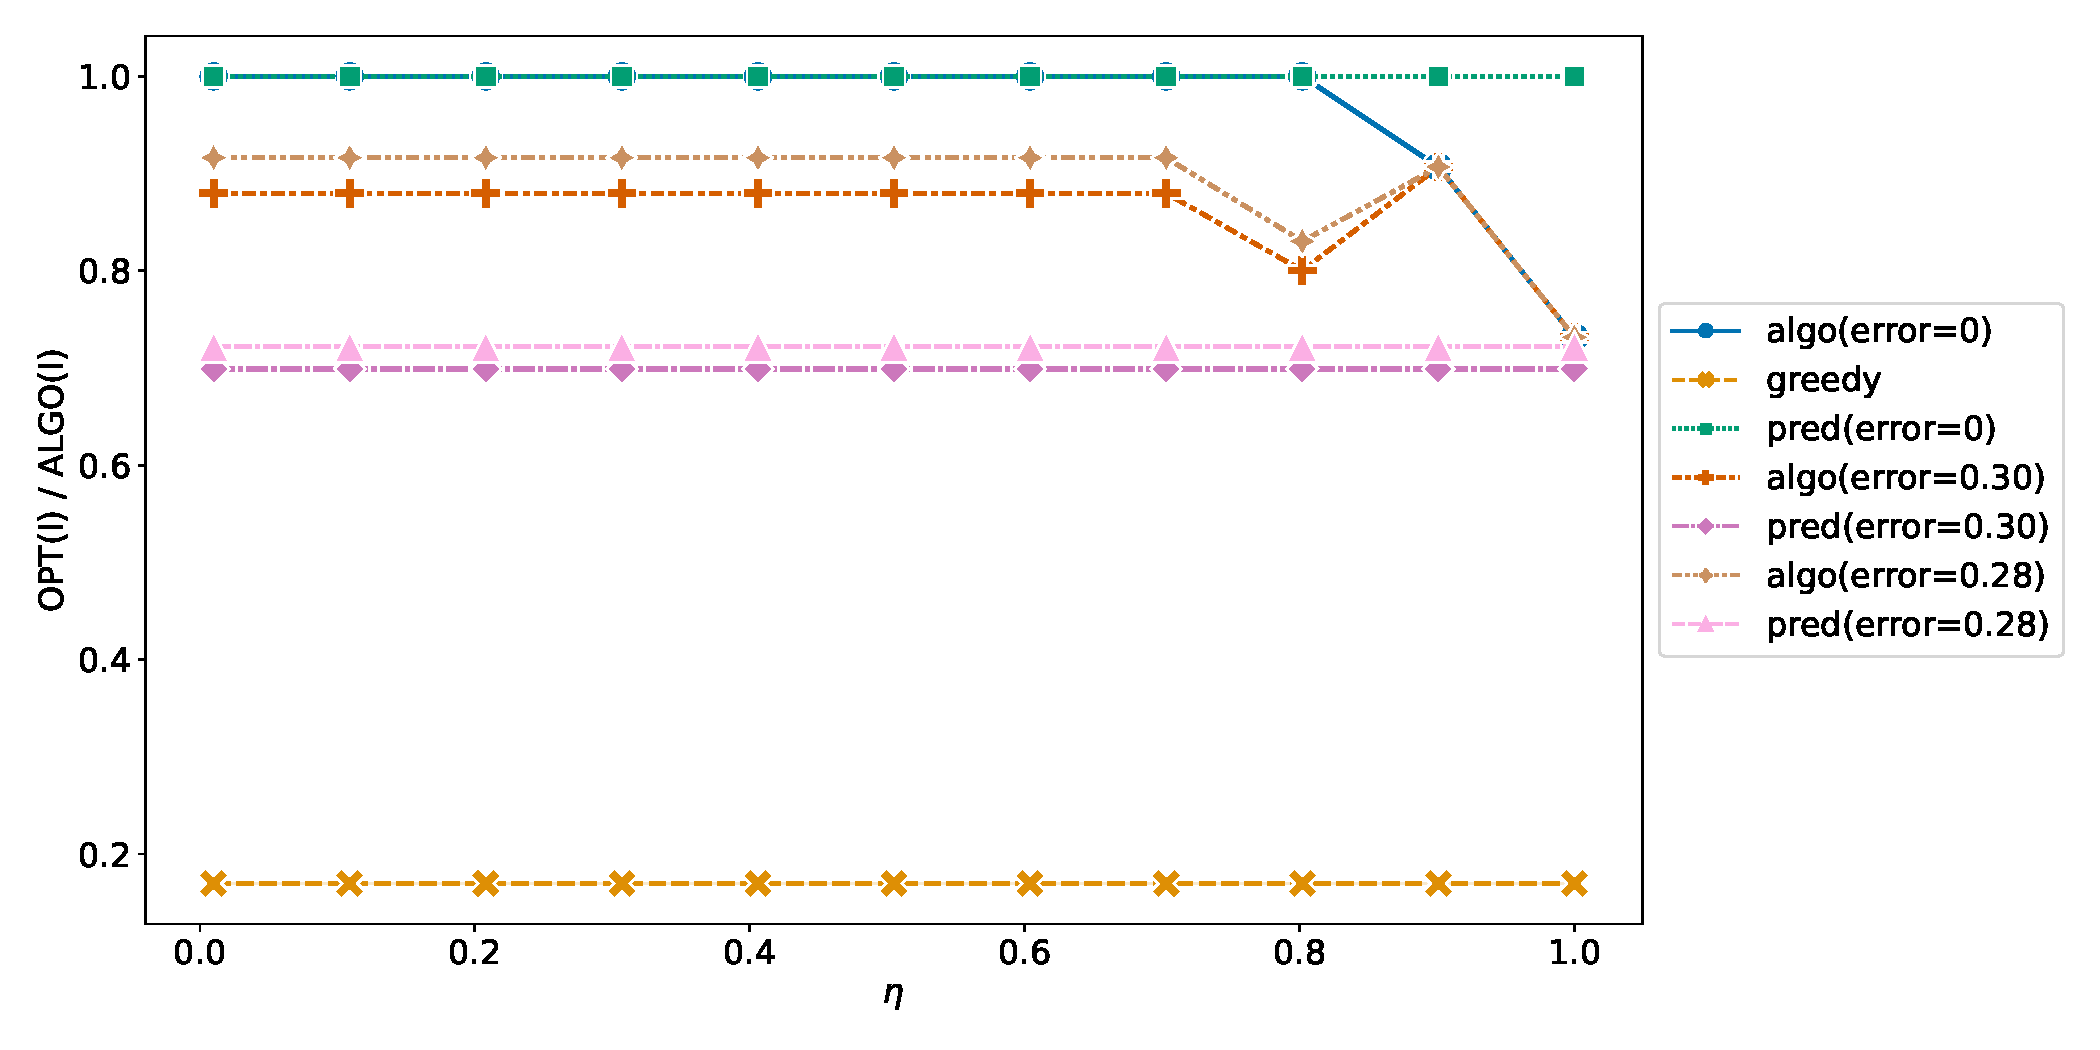
\includegraphics[width=\linewidth]{Img/figure2.pdf}
    \caption{Experiment result. The x-axis show the confidence in the prediction, where 0 means higher confidence. The y-axis show the competitive ratio compared to the optimal offline integral solution. The different colors (also markers) show the result of the algorithm with different prediction error rates and the solutions of the greedy algorithm and the prediction alone. The input graph has $20$ vertices, $69$ arcs, and $10$ requests.}
    \label{fig:experiment-2}
\end{figure}

\begin{figure}[!ht]
    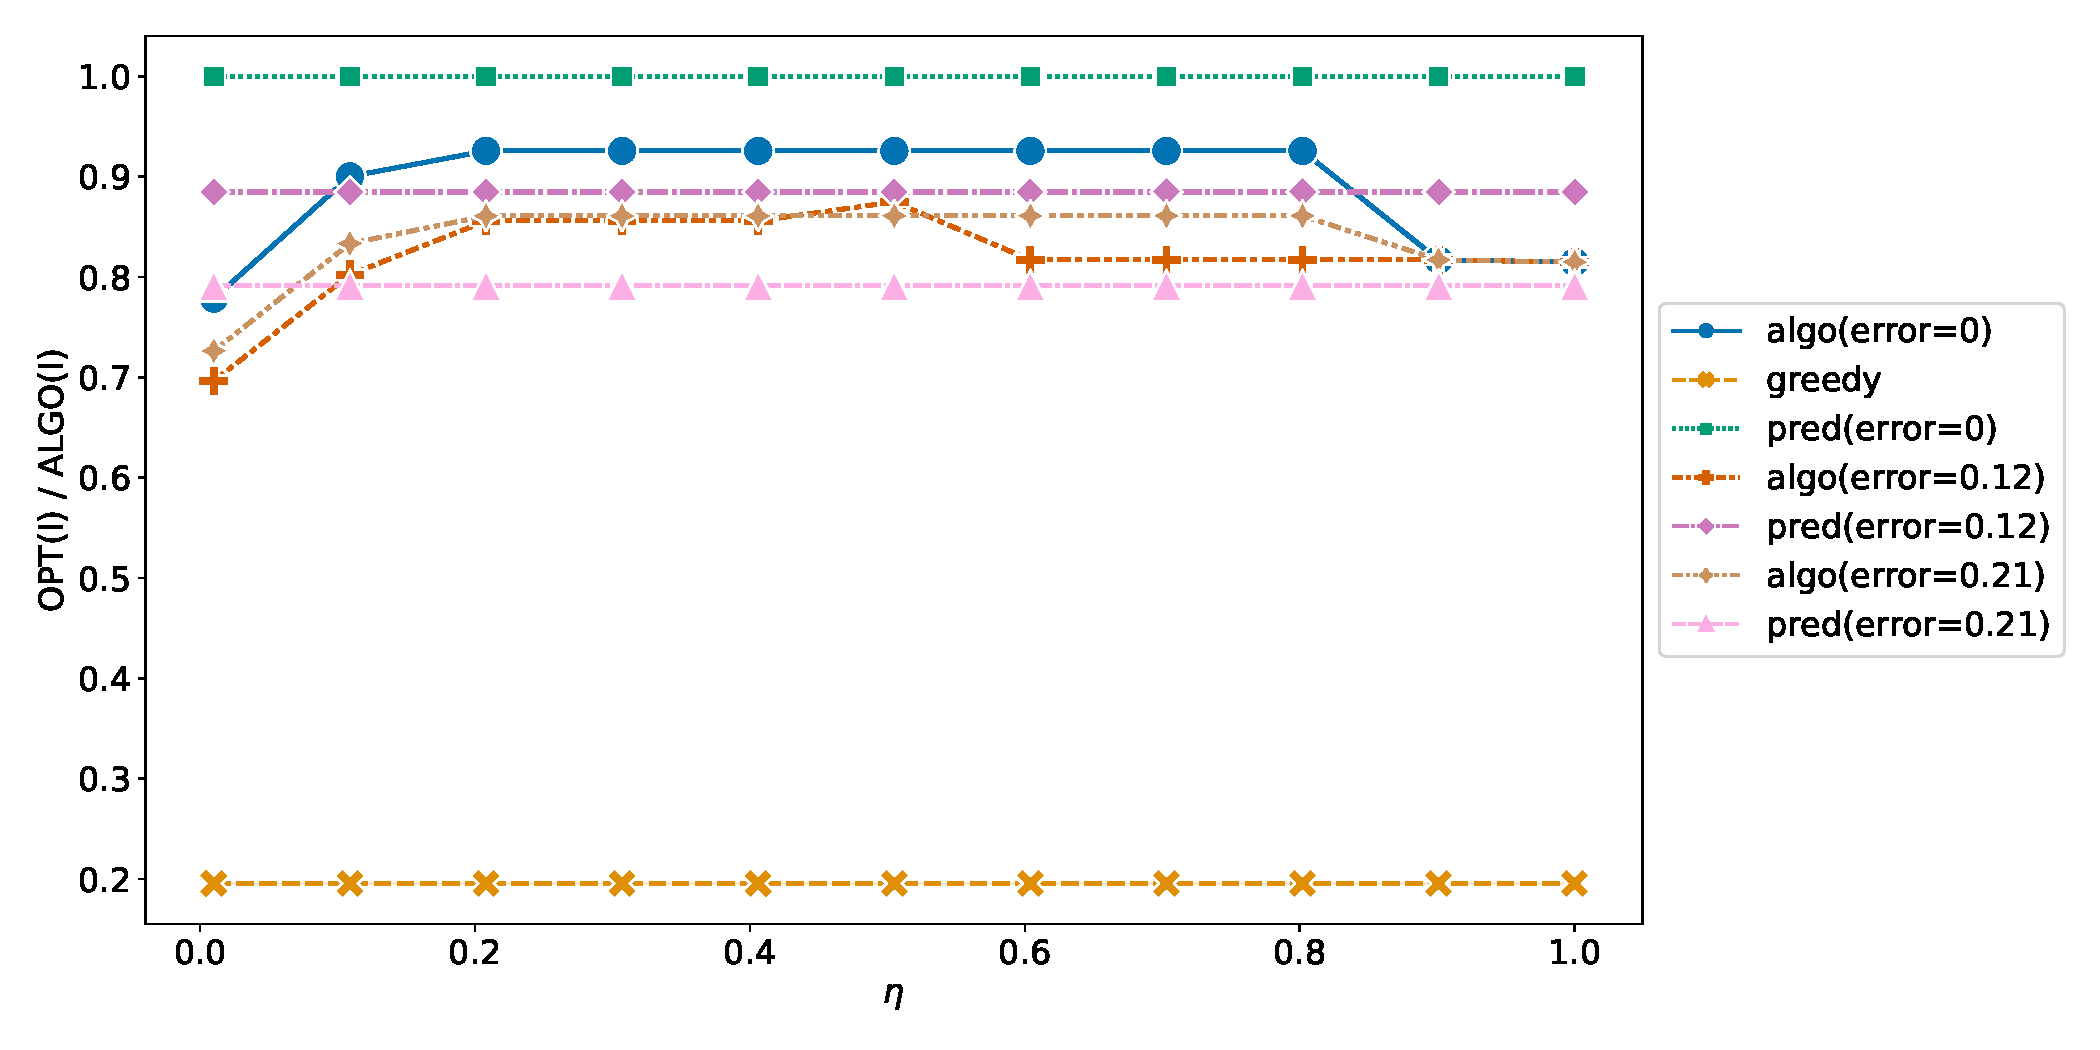
\includegraphics[width=\linewidth]{Img/figure3.pdf}
    \caption{Experiment result. The x-axis show the confidence in the prediction, where 0 means higher confidence. The y-axis show the competitive ratio compared to the optimal offline integral solution. The different colors (also markers) show the result of the algorithm with different prediction error rates and the solutions of the greedy algorithm and the prediction alone. The input graph has $30$ vertices, $73$ arcs, and $20$ requests.}
    \label{fig:experiment-3}
\end{figure}


\end{document}
